\documentclass[12pt,
               color={usenames,   
                      dvipsnames},% Since beamer loads color package 
                                  %  automatically \usepackage{color}   
                                  %  cannot be used to pass options.
%             draft,             % Draft WIP version without header &
%                                  %  footer. Faster compilation.
%               handout,           % Handout version. not sure what it does.
%              notes              % To print notes.
                    ]{beamer}   

%\includeonlyframes{FR_MOTIVE} %FR_PROBLEMS} %FR_EX_IMAGE,FR_EX_TERM}              
                                 %  Use when drafting for fast compile
                                 % turnaround time. 

%%%%%%%%%%%%%%%%%%%%%%%%%%%%%%%%%%%%%%%%%%%%%%%%%%%%%%%%%%%%%%%%%%%%%%%%%%%%%
% Theme customization

\usetheme[compress]{Ilmenau}    % Small circle based TOC on top bar
                                %  single line.
%\usetheme[width=1in]{Hannover}  % TOC left side bar.
%\usetheme{Szeged}               % Similar to Ilmenau except borders on
%                                %  top bar and bottom.
%\usecolortheme  {beetle}        % Grey and blue based.
\useinnertheme  {circles}       % Circle dingbats with no shading.
\usefonttheme[onlylarge]
                {structurebold} % Structure fonts are
                                % bold. Set to only the title / big
                                % fonts.
%\useoutertheme[compress,
%               footline=empty]
%               {miniframes}     % Don't use with explicit themes 

% Beamer elements customization: setbeamercolor/-font/-template
\setbeamercolor{title}                {fg=light3,bg=light1}
\setbeamercolor{subtitle}             {fg=dark1,bg=light1}
\setbeamercolor{date}                 {fg=dark1}
\setbeamercolor{institute}            {fg=dark1}
\setbeamercolor{frametitle}           {fg=dark1,bg=light1}
\setbeamercolor{framesubtitle}        {fg=light5}
\setbeamercolor{structure}            {fg=dark1}
\setbeamercolor{palette primary}      {fg=light1,bg=light2} % Palette
                                              % primary, secondary,
                                              % tertiary, quaternary
                                              % for headline and
                                              % footline 
\setbeamercolor{palette secondary}    {fg=dark2,bg=light3}
\setbeamercolor{palette tertiary}     {fg=light1,bg=light3} 
\setbeamercolor{palette quaternary}   {fg=light1,bg=light2} 
\setbeamercolor{normal text}          {fg=dark2,bg=light1} 
%\setbeamercolor{block body alerted}   {fg=white} %isn't working
\setbeamercolor{alerted text}         {fg=white} % contrast}  %light3} 
\setbeamercolor{block body}           {bg=light5}
\setbeamercolor{block title}          {fg=light1} %,bg=light3} % Uncomment 
                                              % for different block
                                              % heading background

% \setbeamertemplate{blocks}[rounded] % Blocks are rounded on the
%                                     % corners
\setbeamertemplate{blocks}[default] % Blocks are not rounded on the
                                    % corners

\setbeamerfont{framesubtitle}{series={\fontseries{c}}} % Condensed
                                %shape=\sc             % Small caps

%%%%%%%%%%%%%%%%%%%%%%%%%%%%%%%%%%%%%%%%%%%%%%%%%%%%%%%%%%%%%%%%%%%%%%%%%%%%%
% Packages used
\usepackage{../lib/mylatexlib}

\usepackage{setspace}
\usepackage{latexsym}
\usepackage{amssymb}
\usepackage{amsfonts}
\usepackage{amsmath}
%\usepackage{epsfig}
%\usepackage{graphicx}
%\usepackage{epstopdf}
\usepackage{algorithm}
\usepackage{algorithmic}
\usepackage{enumerate}
\usepackage[normalem]{ulem}  % Underline. normalem keeps the default
                             % \em to be italics. 
\usepackage{textcomp}

\usepackage{stmaryrd}

%\usepackage{pifont}
%\usepackage{natbib}
%\usepackage[finalnew]{../lib/trackchanges}


%%%%%%%%%%%%%%%%%%%%%%%%%%%%%%%%%%%%%%%%%%%%%%%%%%%%%%%%%%%%%%%%%%%%%%%%%%%%%
% Loading spcial fonts
\DeclareMathAlphabet{\mathpzc}{OT1}{pzc}{m}{it}
\DeclareMathAlphabet{\mathcalligra}{T1}{calligra}{m}{n}


%%%%%%%%%%%%%%%%%%%%%%%%%%%%%%%%%%%%%%%%%%%%%%%%%%%%%%%%%%%%%%%%%%%%%%%%%%%%%
% Color definitions

%% Inspired by Kuler - Vintage Beach Wear -
%% http://kuler.adobe.com/#themeID/1507195 
\definecolor{dark1}      {HTML}{8A866A}   % Goldish gray     
                                          %     [Structure, Block heading]
\definecolor{light1}     {HTML}{FFF0C2}   % Pale amber          
                                          %     [Slide BG] 
\definecolor{light2}     {HTML}{9C968B}     % Gambogeish gray [???]
\definecolor{light3}     {HTML}{A36D5C}   % Grayish vermilion   
                                          %     [Title, Header & footer BG] 
\definecolor{dark2}      {HTML}{473C35}   % Dark grayish tangelo
                                          %     [Slide normal text FG]
\definecolor{light5}     {HTML}{A8A87D}   % Greyish olive
                                          %     [Block BG]
\definecolor{contrast}   {HTML}{197DE5}   % Brilliant azure     
                                          %     [Stark Contrast]



%%%%%%%%%%%%%%%%%%%%%%%%%%%%%%%%%%%%%%%%%%%%%%%%%%%%%%%%%%%%%%%%%%%%%%%%%%%%%
% String defs
\def\cA{{\cal A}}  \def\cB{{\cal B}}  \def\cC{{\cal C}}  \def\cD{{\cal D}}
\def\cE{{\cal E}}  \def\cF{{\cal F}}  \def\cG{{\cal G}}  \def\cH{{\cal H}}
\def\cI{{\cal I}}  \def\cJ{{\cal J}}  \def\cK{{\cal K}}  \def\cL{{\cal L}}
\def\cM{{\cal M}}  \def\cN{{\cal N}}  \def\cO{{\cal O}}  \def\cP{{\cal P}}  
\def\cQ{{\cal Q}}  \def\cR{{\cal R}}  \def\cS{{\cal S}}  \def\cT{{\cal T}}  
\def\cU{{\cal U}}  \def\cV{{\cal V}}  \def\cW{{\cal W}}  \def\cX{{\cal X}}
\def\cY{{\cal Y}}  \def\cZ{{\cal Z}}  \def\hA{{\hat A}}  \def\hB{{\hat B}}
\def\hC{{\hat C}}  \def\hD{{\hat D}}  \def\hE{{\hat E}}  \def\hF{{\hat F}}
\def\hG{{\hat G}}  \def\hH{{\hat H}}  \def\hI{{\hat I}}  \def\hJ{{\hat J}}
\def\hK{{\hat K}}  \def\hL{{\hat L}}  \def\hP{{\hat P}}  \def\hQ{{\hat Q}}
\def\hR{{\hat R}}  \def\hS{{\hat S}}  \def\hT{{\hat T}}  \def\hX{{\hat X}}
\def\hY{{\hat Y}}  \def\hZ{{\hat Z}}
\def\A{{\mathcal A}}  \def\bI {\mathbb I}
\def\C{{\mathcal C}}  \def\bO {\mathbb O}
\def\F{{\mathcal F}}  \def\cl {\mathpzc{l}}
\def\H{{\mathcal H}}  \def\cg {\mathpzc{g}}
                      \def\ccT{\mathpzc{T}}

\def\overlap   {\between}
\def\eps       {\epsilon}
\def\icppl     {\maltese} 
\def\invb      {\textreferencemark}
\def\assign    {\leftarrow}

\def\lndisplay      {1}
\def\commentboxsize {7cm}
\def\prelimspace    {2mm}
\def\alertseccolor {contrast}

% For BibTeX formatting \newblock
\def\newblock{\hskip .11em plus .33em minus .07em}
% for Natbib
%\bibpunct{(}{)}{;}{a}{,}{,}


% %%%%%%%%%%%%%%%%%%%%%%%%%%%%%%%%%%%%%%%%%%%%%%%%%%%%%%%%%%%%%%%%%%%%%%%%%%%%%
% % New/renew commands
% % Format of comments in algorithmic package
% \renewcommand{\algorithmiccomment}[1]
% { 
%   \vspace {0.5mm}
%   \hfill
%   {\small
%   \begin{tabular}{|r}
%     \parbox[right]{\commentboxsize}{ \space \tt{ #1 }}\\  
%     % {\tt /* #1 */} \hspace{2mm}
%   \end{tabular}
%   }
% }


% % Theorems etc. 
% \newtheorem{observation}{Observation}
%%% 1 DEC
% \newcommand{\seq}[1]{\left\langle #1 \right\rangle}
% \newcommand{\set}[1]{\left\{ #1\right\}}
% \newcommand{\supp}[1]{supp\left( #1 \right)}
%%% END 1 DEC

%%%%%%%%%%%%%%%%%%%%%%%%%%%%%%%%%%%%%%%%%%%%%%%%%%%%%%%%%%%%%%%%%%%%%%%%%%%%%
% Title slide details
\title[{\bf tree path labeling} -- a generalization of consecutive
       ones property of binary matrices]
         {Tree Path Labeling of\\ Path Hypergraphs}
\subtitle{A Generalization of Consecutive Ones Property}

\author[anju s $|$ \tt{anjuzabil@gmail.com}]{Anju Srinivasan}

\institute[CS09S012]
         {as part of {\bf M.\;S.} by Research \\ 
          advised by {\bf Dr.\;N.\;S.\;Narayanaswamy}\\ 
          CSED, IITM, Chennai - 36}

\date{25 Mar 2013}


%%%%%%%%%%%%%%%%%%%%%%%%%%%%%%%%%%%%%%%%%%%%%%%%%%%%%%%%%%%%%%%%%%%%%%%%%%%%%
% Document begins

\begin{document}

\frame{
 \titlepage
}
\section*{Outline}
\frame{
  \tableofcontents % [pausesections]
}

\section{Introduction}

\subsection{Motivation}
\frame<1>[label=FR_MOTIVE]{
  \frametitle{Motivation}
%  \framesubtitle{consecutive ones is a special case of tree path labeling}

  \begin{block}{}
 {\footnotesize
  \begin{tabular}{cccc c}
    &&\textcolor{dark1}{Combinatorial}& & \\
    &&\textcolor{dark1}{algorithms}&&\\
    && \textcolor{dark1}{$\downarrow$} &     &\\
    && \textcolor{dark1}{Matrix reordering} &     & \only<2-> {Tree canonization}\\
    && \textcolor{dark1}{problems} && \only<2->{\tiny \cite{sl92}}\\
    && \textcolor{dark1}{$\downarrow$} &&\only<2->{$\downarrow$}\\    

    Interval &$\leftrightharpoons$& \textcolor{light3}{ {\bf Consecutive
      Ones} } &\only<2->{$\Longmapsto$}& \only<2->{ Interval graph}\\
    labeling&& \textcolor{light3}{\bf Property} && \only<2->{
      canonization}\\
    {\tiny \cite{kklv10}}&&{\tiny \textcolor{light3}{ \bf \cite{fg65,at72,bl76,nsnrs09}}}&&\only<2->{\tiny \cite{kklv10}}\\

    $\Downarrow$&&&&\only<2->{$\Downarrow$}\\

    \textcolor{light3}{\bf Tree Path}&&\only<3>{ \textcolor{red}{Path graph}}&& \only<2->{ Interval graph}\\
    \textcolor{light3}{\bf Labeling}&\only<3>{$\Longmapsto$}&\only<3>{ \textcolor{red}{canonization}}&& \only<2->{ isomorphism}\\
    
    &&\only<3>{$\Downarrow$}&& \only<2->{\tiny \cite{kklv10}}\\
    &&\only<3>{ \textcolor{red}{Path graph}}&& \\
    &&\only<3>{ \textcolor{red}{isomorphism}}&& 
  \end{tabular}
 }

  \end{block}

}

% \frame{
% \tnote{A 30 sec slide on COP? TBD IN THE END}
% }


\subsection{An Illustration}

\frame[label=FREXAMPLE]{
  \frametitle{}
  \begin{overlayarea}{\textwidth}{1cm}
    
    \begin{centering}
      \only<1->{\Huge An Illustration}
    \end{centering}

    \begin{centering}
      \only<2>{of Tree Path Labeling problem}
    \end{centering}
  \end{overlayarea}
}

% \frame[label=FREXAMPLE2]{
%   \frametitle{A Study Group Housing problem}
% % \begin{centering}

%   \tnote{update to the example in synopsis doc}
  
%   \begin{itemize}[<uncover@+->]
%   \item A set of $n$ students arrive for a summer course, say
%     $\{a,b,c,d,e,f,g,h,i,j,k\}$, $n= 11$.
%   \item They form $m$ study groups, say $\{\textcolor{red}{R},
%     \textcolor{blue}{B}, \textcolor{orange}{O},
%     \textcolor{green}{G}\}$, $m = 4$
%   \item A student may be in more than one study group but {\bf will} be in
%     at least one, say
%     \begin{itemize}
%     \item $\textcolor{red}{R = \{g, h, i, j, k\}}$
%     \item $\textcolor{blue}{B = \{a, b, e, g\}}$
%     \item $\textcolor{orange}{O = \{c, b, d\}}$
%     \item $\textcolor{green}{G = \{e, f , g, i\}}$
%     \end{itemize}

%   \item There are $n$ single occupancy apartments in the university campus for their accommodation.
%   \item All these apartments are placed such that streets connecting
%     them do not form loops
%   \end{itemize}

% %\note{}  
% %  \end{centering}
% }

\def \Pa {{\em {\bf Pa}tricia}} 
\def \Pi {{\em {\bf Pi}gpen}}
\def \Sn {{\em {\bf Sn}oopy}}
\def \Wo {{\em {\bf Wo}odstock}}
\def \Vi {{\em {\bf Vi}olet}} 
\def \Li {{\em {\bf Li}nus}} 
\def \Ch {{\em {\bf Ch}arlie}}
\def \Sa {{\em {\bf Sa}lly}}
\def \Fr {{\em {\bf Fr}anklin}} 
\def \Sc {{\em {\bf Sc}hr{\"o}eder}} 
\def \Lu {{\em {\bf Lu}cy}}
\def \xPa {{\bf Pa}} 
\def \xPi {{\bf Pi}} 
\def \xSn {{\bf Sn}}
\def \xWo {{\bf Wo}}
\def \xVi {{\bf Vi}} 
\def \xLi {{\bf Li}} 
\def \xCh {{\bf Ch}}
\def \xSa {{\bf Sa}}
\def \xFr {{\bf Fr}}
\def \xSc {{\bf Sc}} 
\def \xLu {{\bf Lu}}
\def \residenceblock {{\em Infinite Loop}}
\def \WSI {{\em Wallace Studies Institute}}
\def \coneohone {{\em ``Influence of post modernism in Wallace's work''}}
\def \coneohtwo {{\em ``A study on fragmented prose method''}}

\def \LLL {{\em ``$\mathbb{B}$rief Interviews with Hideous Men''}}
\def \GGG {{\em ``The String $\mathbb{T}$heory''}} 
\def \BBB {{\em ``[$\mathbb{W}$]Rhetoric and the Math Melodrama''}}
\def \TTT {{\em ``$\mathbb{F}$ate, Time, and Language: An Essay on Free Will''}}
\def \clrLLL {red}
\def \clrGGG {blue} 
\def \clrBBB {orange} %{YellowOrange}
\def \clrTTT {green}
\def \xLLL {\textcolor{\clrLLL}{\mathbb{B}}}
\def \xGGG {\textcolor{\clrGGG}{\mathbb{T}}}
\def \xBBB {\textcolor{\clrBBB}{\mathbb{W}}}
\def \xTTT {\textcolor{\clrTTT}{\mathbb{F}}}

\frame[label=FREXAMPLE2]{
  \frametitle{Study Group Accommodation problem}

%   \tnote{ONLY DIAGRAMS.\\
%   a00.pdf - a venn diagram of just the universe\\
%   a0.pdf - a venn diagram of the grouping}
%   \begin{tabular}{cc}
%     $\{\xPa,\; \xPi,\; \xSn,\; \xWo,\; $
%    &
%       \begin{tabular}{rcl}
%         $\xLLL $&$=$&$ \{\xCh,\;  \xSa,\;  \xFr,\;  \xSc,\;  \xLu \}$\\
%         $\xGGG $&$=$&$ \{\xPa,\;  \xPi,\;  \xVi,\;  \xCh \}$\\
%         $\xBBB $&$=$&$ \{\xSn,\;  \xPi,\;  \xWo \}$\\
%         $\xTTT $&$=$&$ \{\xVi,\;  \xLi,\;  \xCh,\;  \xFr \}$\\
%       \end{tabular}
%     \\

%     $\xVi,\; \xLi,\; \xCh,\; \xSa,\; $&&\\
%     $\xFr,\; \xSc,\; \xLu\}$&&

%   \end{tabular}

  \begin{tabular}{cc}

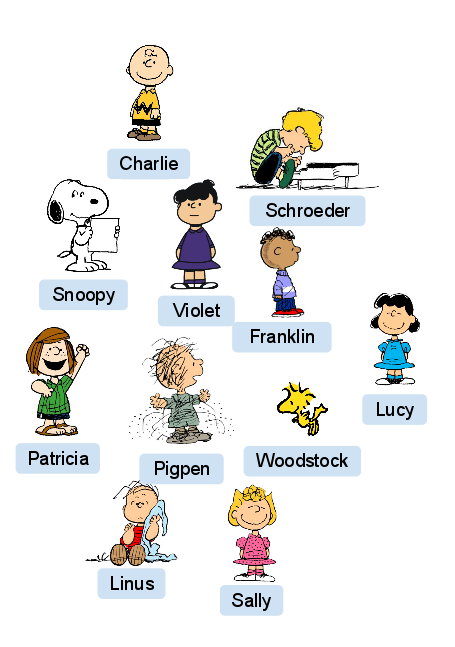
\includegraphics[scale=0.2]{../img/U.png} &
      \begin{tabular}{rcl}
        $\xLLL $&$=$&$ \{\xCh,\;  \xSa,\;  \xFr,\;  \xSc,\;  \xLu \}$\\
        $\xGGG $&$=$&$ \{\xPa,\;  \xPi,\;  \xVi,\;  \xCh \}$\\
        $\xBBB $&$=$&$ \{\xSn,\;  \xPi,\;  \xWo \}$\\
        $\xTTT $&$=$&$ \{\xVi,\;  \xLi,\;  \xCh,\;  \xFr \}$\\
      \end{tabular}\\
      Students & Study groups
  \end{tabular}

%   \note{
% %  \begin{block}{} 
%   \begin{itemize}%[<uncover@+->]
%   \item A set of {$n$ students} arrive for a summer course, say
%     { $\{\xPa,\; \xPi,\; \xSn,\; \xWo,\; \xVi,\; \xLi,\; \xCh,\;
%     \xSa,\; \xFr,\; \xSc,\; \xLu\}$, $n= 11$}
%   \item They form {$m$ study groups}, say {$\{\xLLL,
%       \xGGG, \xBBB, \xTTT\}$, $m = 4$}
%   \end{itemize}
% %  \end{block}
%   }
}


\frame[label=FREXAMPLE3]{
  \frametitle{Study Group Accommodation problem}

  \only<1>
  {
  \begin{tabular}{c|c}
          \begin{tabular}{rcl}
        $\xLLL $&$=$&$ \{\xCh,\;  \xSa,\;  \xFr,\;  \xSc,\;  \xLu \}$\\
        $\xGGG $&$=$&$ \{\xPa,\;  \xPi,\;  \xVi,\;  \xCh \}$\\
        $\xBBB $&$=$&$ \{\xSn,\;  \xPi,\;  \xWo \}$\\
        $\xTTT $&$=$&$ \{\xVi,\;  \xLi,\;  \xCh,\;  \xFr \}$\\
      \end{tabular}\\
    &
    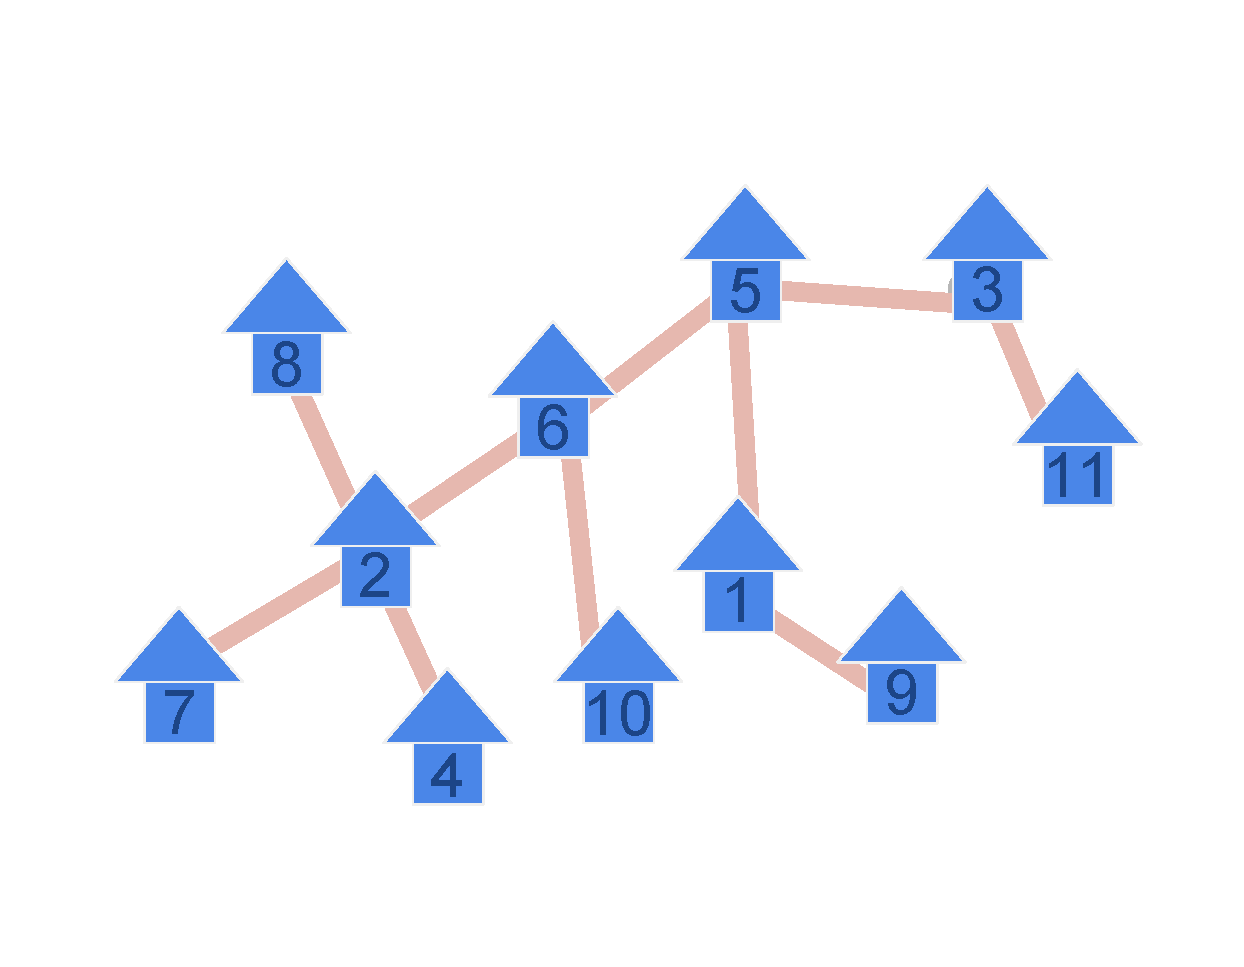
\includegraphics[scale=0.2]{../img/1_infinite_loop.pdf}\\%{a1.pdf}\\
    
    {\small Study groups}&
    {\small {\residenceblock } residential block}
  \end{tabular}
  }

  \only<2>
  {
  \begin{tabular}{c|c}
    {\tiny
      \begin{tabular}{rcl}
        $\xLLL $&$=$&$ \{\xCh,\;  \xSa,\;  \xFr,\;  \xSc,\;  \xLu \}$\\
        $\xGGG $&$=$&$ \{\xPa,\;  \xPi,\;  \xVi,\;  \xCh \}$\\
        $\xBBB $&$=$&$ \{\xSn,\;  \xPi,\;  \xWo \}$\\
        $\xTTT $&$=$&$ \{\xVi,\;  \xLi,\;  \xCh,\;  \xFr \}$\\
      \end{tabular}
    }
&
    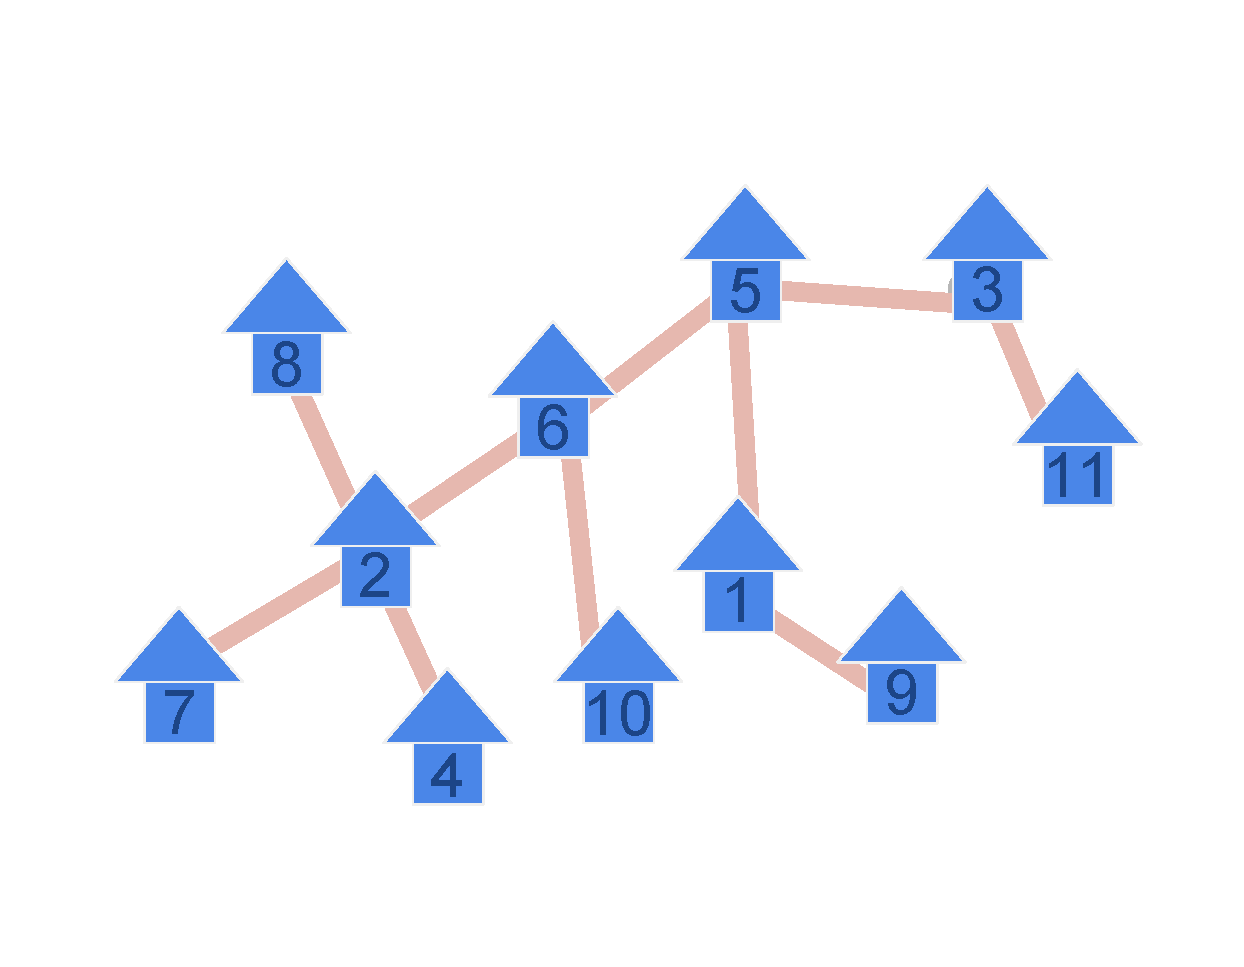
\includegraphics[scale=0.1]{../img/1_infinite_loop.pdf}\\
    
    {\small Study groups}&
    {\small {\residenceblock } residential block}
  \end{tabular}
  }



  \begin{block}<2>{}
    \begin{itemize}
    \item A student may be in more than one study group but {will be
        in at least one}.
    \item There are equal number of {single occupancy apartments} in
      \residenceblock.
    \item Streets connecting them {do not} form loops.
    \end{itemize}
    
  \end{block}


%   \note{
%     \begin{itemize}
%     \item A student may be in more than one study group but {will be
%         in
%         at least one}, say \\
%       \begin{tabular}{rcl}
%         $\xLLL $&$=$&$ \{\xCh,\;  \xSa,\;  \xFr,\;  \xSc,\;  \xLu \}$\\
%         $\xGGG $&$=$&$ \{\xPa,\;  \xPi,\;  \xVi,\;  \xCh \}$\\
%         $\xBBB $&$=$&$ \{\xSn,\;  \xPi,\;  \xWo \}$\\
%         $\xTTT $&$=$&$ \{\xVi,\;  \xLi,\;  \xCh,\;  \xFr \}$\\
%       \end{tabular}
%     \item There are {$n$ single occupancy apartments} in
%       \residenceblock.
%     \item Streets connecting them {do not form loops.}
%     \end{itemize}
%   }
}


\frame[label=FR_EX_PROB]{
  \framesubtitle{}
  {\center \Huge The problem}

  \begin{block}{}
    \begin{centering}
    {How should the students be allocated apartments such that
    \alert{students in each group should inhabit a (continuous) path}?} 
    \end{centering}    
  \end{block}

%   \begin{block}<2->{Additional condition}
%     \begin{centering}
%     \begin{overlayarea}{\textwidth}{1cm}
%       {\\}
%       \only<3>{Else, it is \em a subtree labeling problem} (out of
%       scope).
%     \end{overlayarea}
%     \end{centering}
%   \end{block}

}


\frame[label=FR_EX_IMAGE]{
  \frametitle{Allocate \textcolor{light3}{Paths} to
    \textcolor{light3}{Study Groups}} 
  \framesubtitle{tree path labeling \only<4>{- feasible?}}

  %% Frames 2,3,4
  {
    \begin{tabular}{cc}
      %% Show a0, a1 at overlay 2
      \only<2-3>{
       {\tiny
      \begin{tabular}{rcl}
        $\xLLL $&$=$&$ \{\xCh,\;  \xSa,\;  \xFr,\;  \xSc,\;  \xLu \}$\\
        $\xGGG $&$=$&$ \{\xPa,\;  \xPi,\;  \xVi,\;  \xCh \}$\\
        $\xBBB $&$=$&$ \{\xSn,\;  \xPi,\;  \xWo \}$\\
        $\xTTT $&$=$&$ \{\xVi,\;  \xLi,\;  \xCh,\;  \xFr \}$\\
      \end{tabular}}

        & 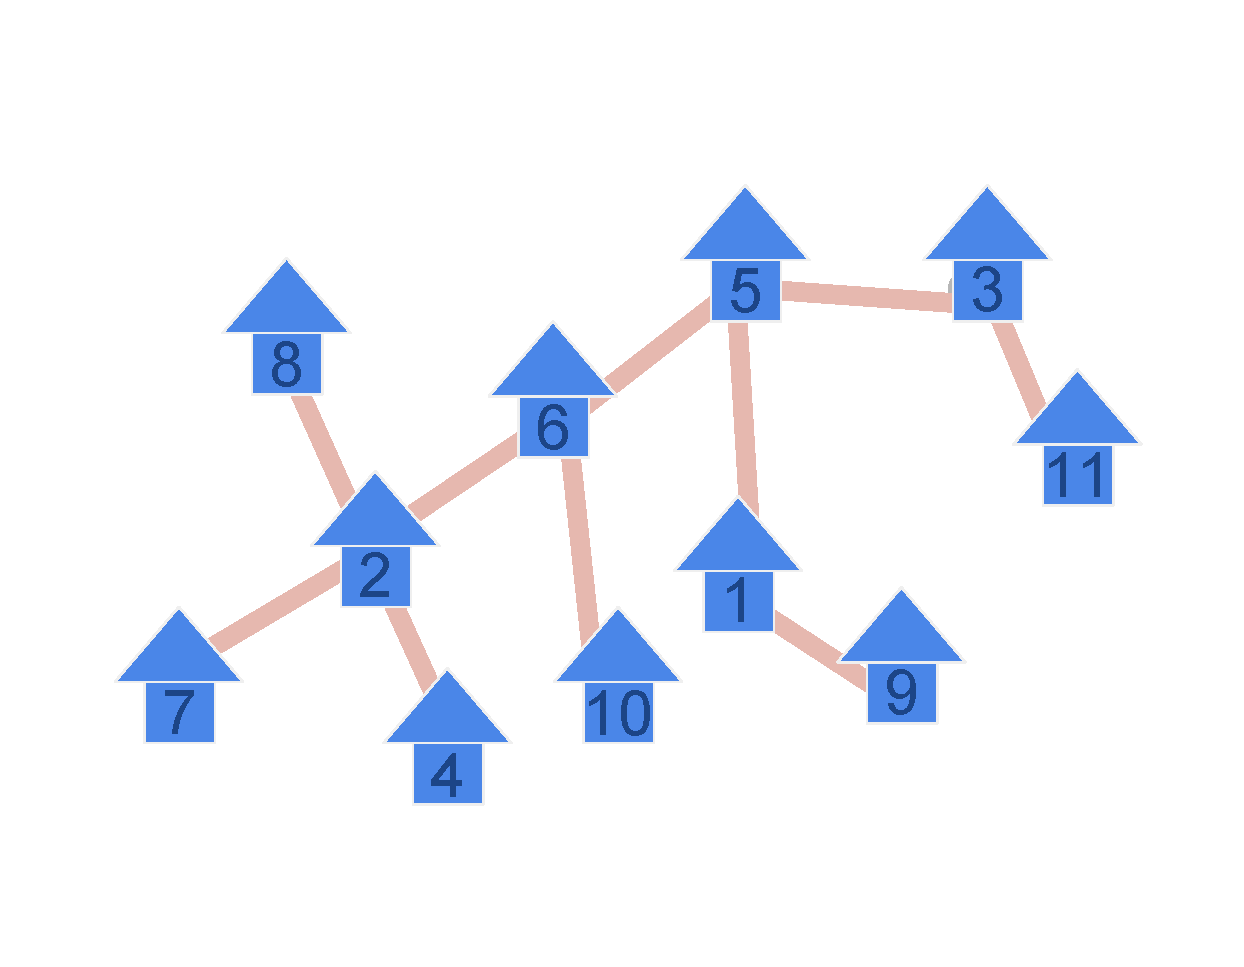
\includegraphics[scale=0.1]{../img/1_infinite_loop.pdf}

        \\}

      %% Show a0, a1 at overlay 3
      \only<3-4>{
        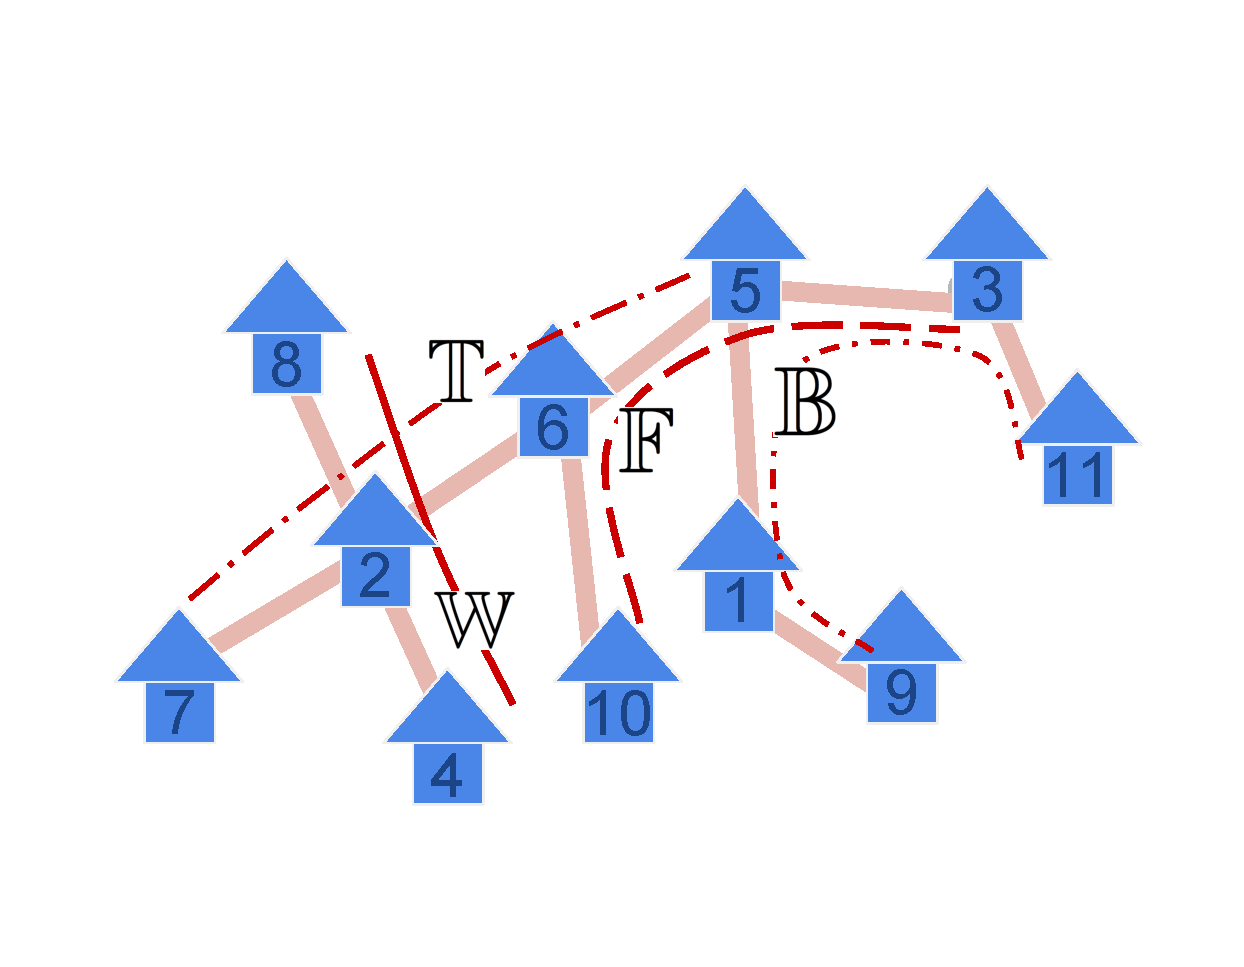
\includegraphics[scale=0.2]{../img/2_infinite_loop_BTWF.pdf}%{a2.pdf}
      } & 
      \only<4> {\bf Is this feasible? }\\
      \only<2-3> {Study groups - ${\xLLL}, {\xGGG}, {\xBBB}, {\xTTT}$}&
    \end{tabular}
  }

%   %% Frames 5,6,7
%   {
%     \begin{tabular}{cc}
%       %% Show a2, a0 at overlay 5
%       \only<5-7>{
%         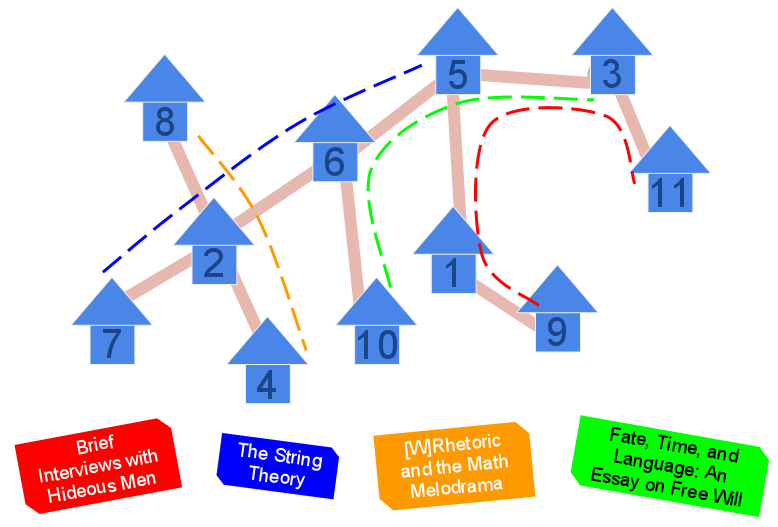
\includegraphics[scale=0.1]{../img/2_infinite_loop_BTWF.png} 
%         \tnote{replace with udpated.}
%         & \tnote{a0.pdf} 
%         \\}

%       %% Show a0, a1 at overlay 3
%       \only<6> {In this case, IS feasible.&}
      
%       \only<7>{
%         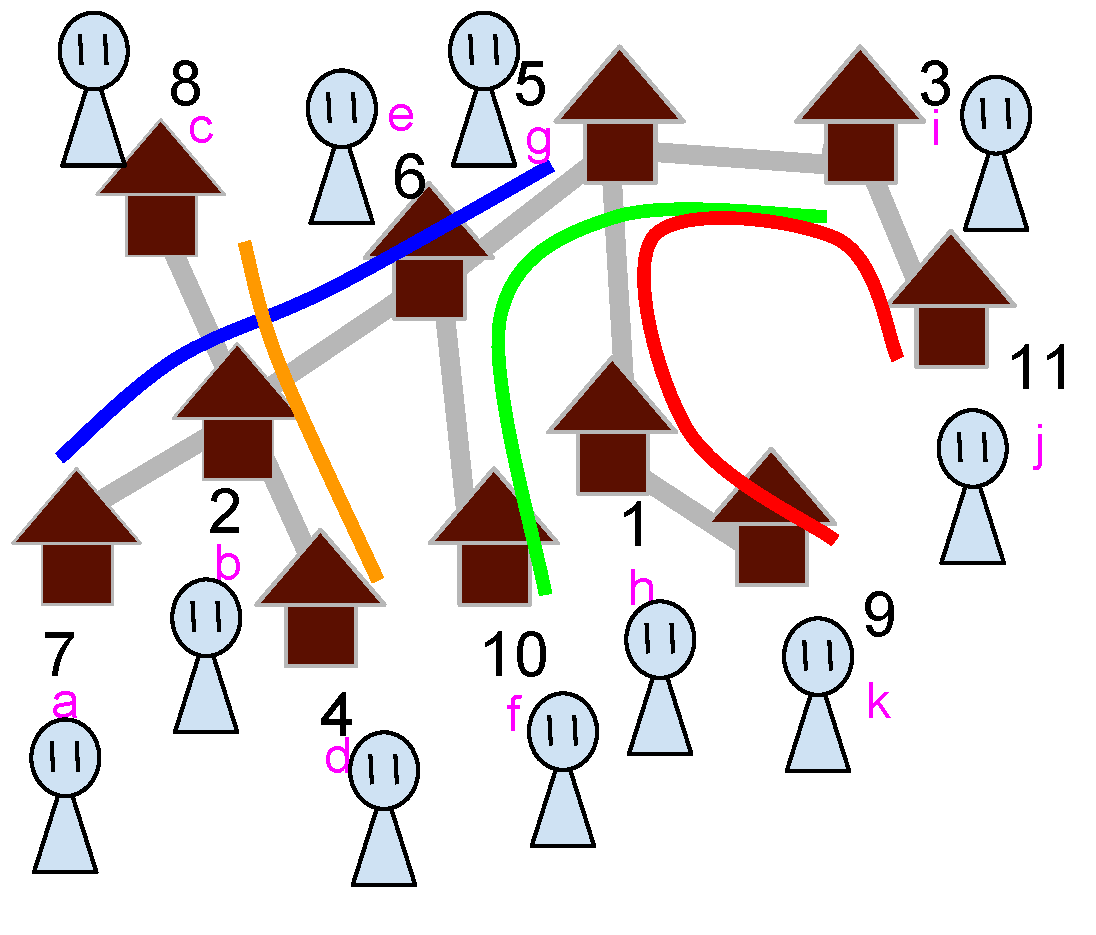
\includegraphics[scale=0.35]{a3.pdf}&
%       } 
      
%     \end{tabular}
%   }
}


\frame[label=FR_EX_IMAGE]{
  \frametitle{Allocate \textcolor{light3}{Apartments} to
    \textcolor{light3}{Students}} 
  \framesubtitle{path graph isomorphism/feasibility bijection}

%   %% Frames 2,3,4
%   {
%     \begin{tabular}{cc}
%       %% Show a0, a1 at overlay 2
%       \only<2-3>{
%         \tnote{a0.pdf} 
%         & 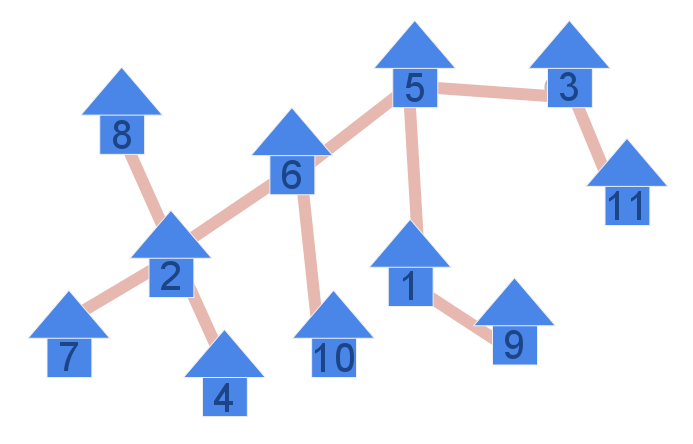
\includegraphics[scale=0.1]{../img/1_infinite_loop.png}
%         \tnote{replace with udpated.}
%         \\}

%       %% Show a0, a1 at overlay 3
%       \only<3-4>{
%         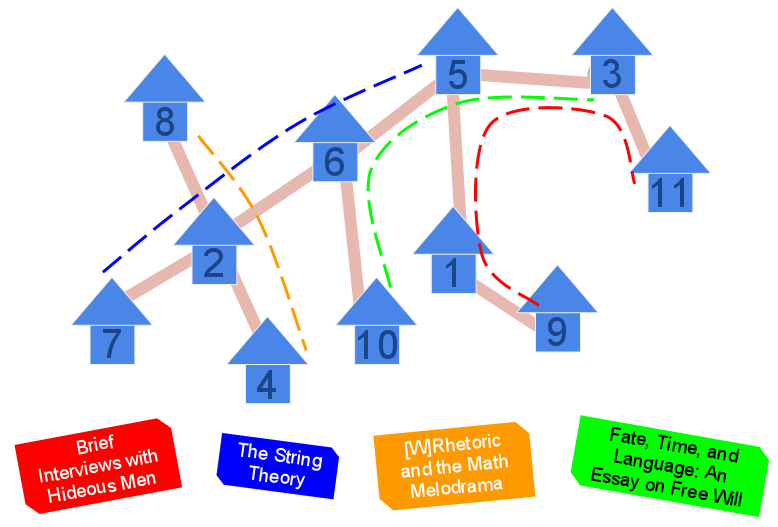
\includegraphics[scale=0.35]{../img/2_infinite_loop_BTWF.png}
%       } & 
%       \only<4> {Is this feasible?}
%     \end{tabular}
%   }

  %% Frames 5,6,7
  {
    \begin{tabular}{cc}
      %% Show a2, a0 at overlay 5
      \only<2-4>{ %<5-7>{
        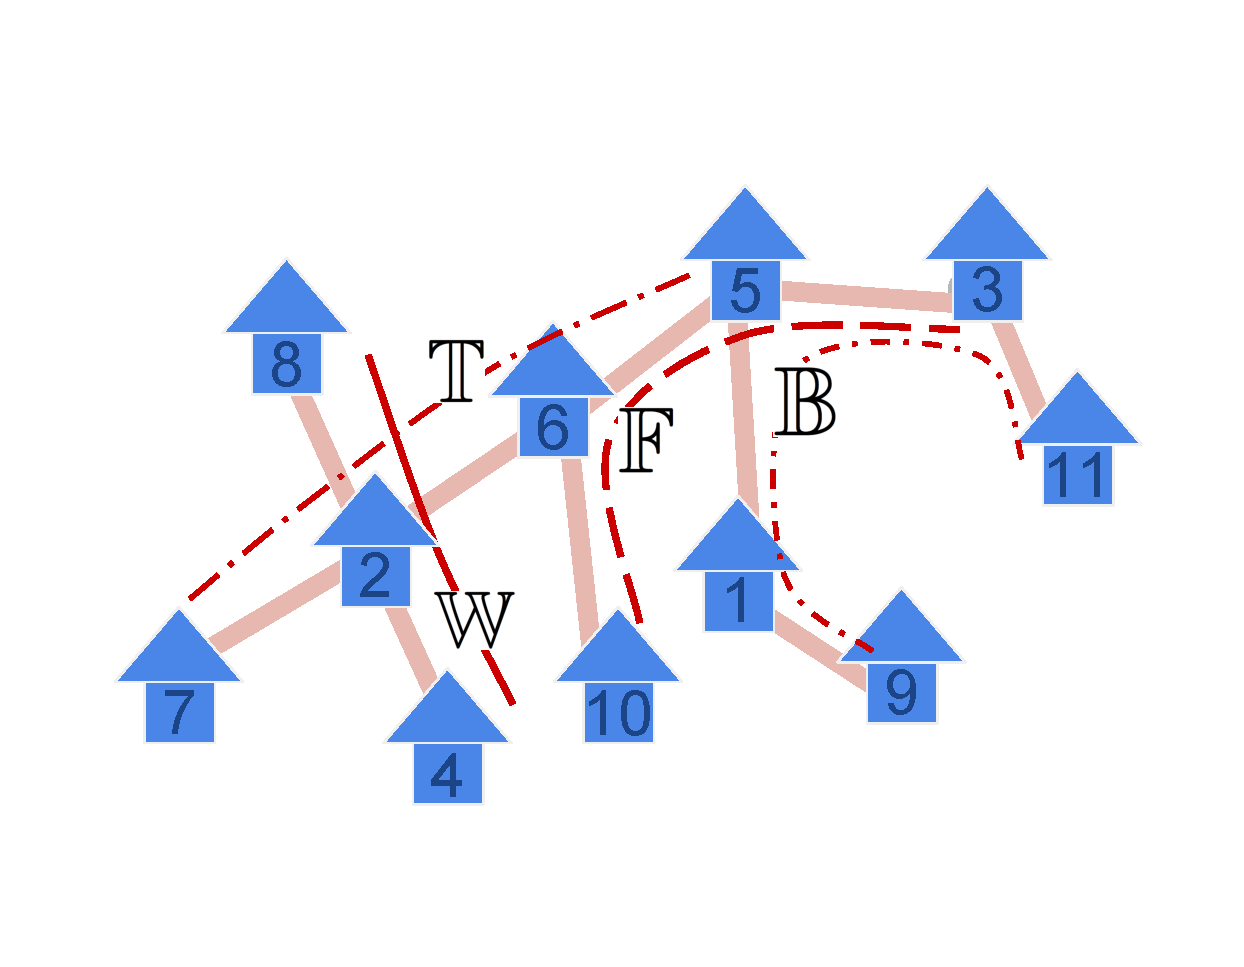
\includegraphics[scale=0.1]{../img/2_infinite_loop_BTWF.pdf} 
        & 
      \begin{tabular}{rcl}
        $\xLLL $&$=$&$ \{\xCh,\;  \xSa,\;  \xFr,\;  \xSc,\;  \xLu \}$\\
        $\xGGG $&$=$&$ \{\xPa,\;  \xPi,\;  \xVi,\;  \xCh \}$\\
        $\xBBB $&$=$&$ \{\xSn,\;  \xPi,\;  \xWo \}$\\
        $\xTTT $&$=$&$ \{\xVi,\;  \xLi,\;  \xCh,\;  \xFr \}$\\
      \end{tabular}\\
        \\}

      %% Show a0, a1 at overlay 3
      \only<3> %<6> 
      {  In this case, \textcolor{light3}{\bf is feasible}.&}
      \only<4>
      {  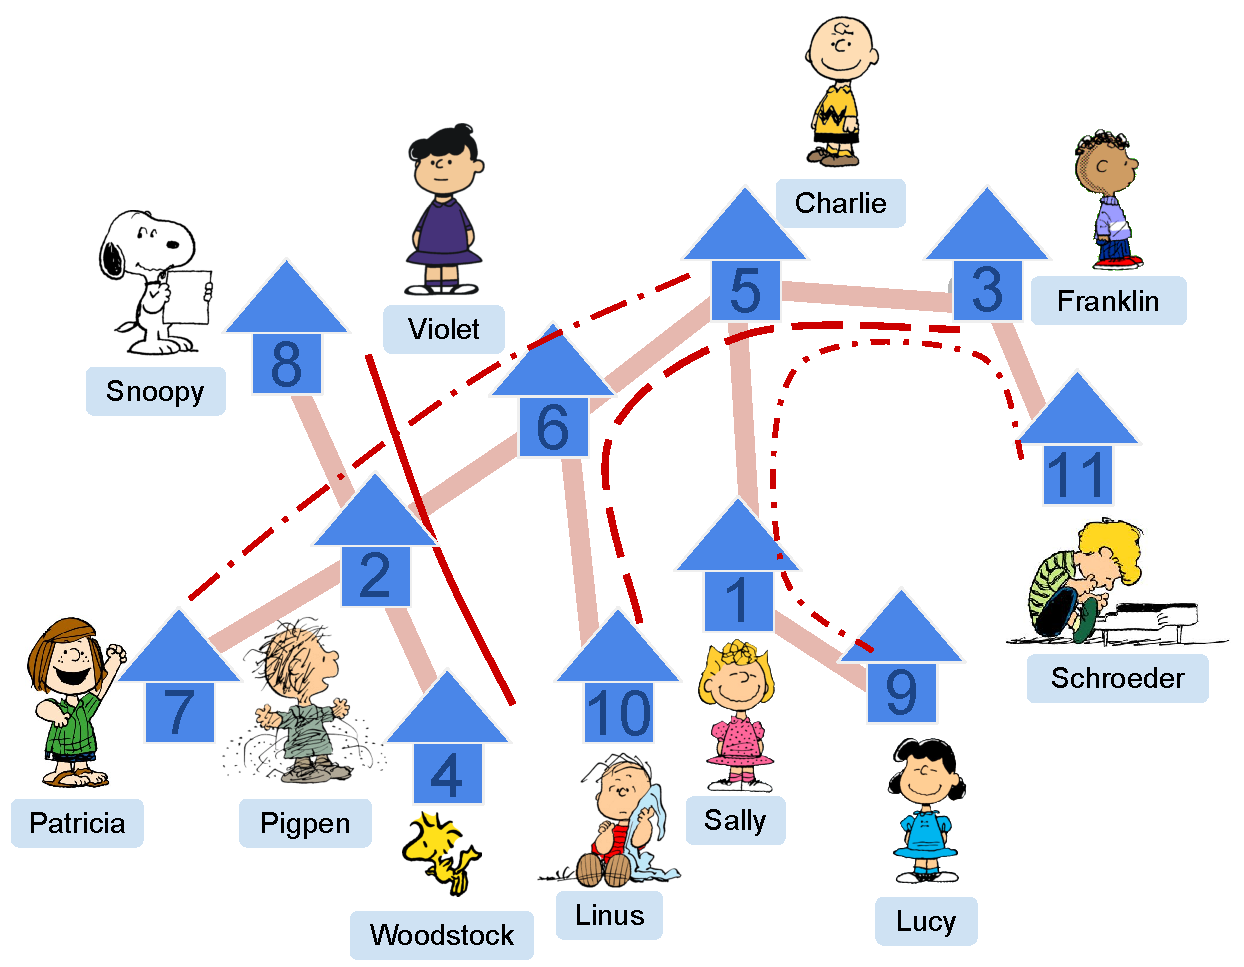
\includegraphics[scale=0.1]{../img/3_infinite_loop.pdf}&} %{a3.pdf}
    \end{tabular}
  }
}


\def \termimgscale {0.25}

\frame[label=FR_EX_TERM]{ 
  \frametitle{Basic terminology} 
  \framesubtitle{a crash course on the TPL machinery}

  \only<2>{

    \begin{block}{}
      The set of study groups $\{\xLLL,
      \xGGG, \xBBB, \xTTT\}$ $\rightarrow$
      \alert{\sc Hypergraph}
    \end{block}
  }

  \only<3>{
    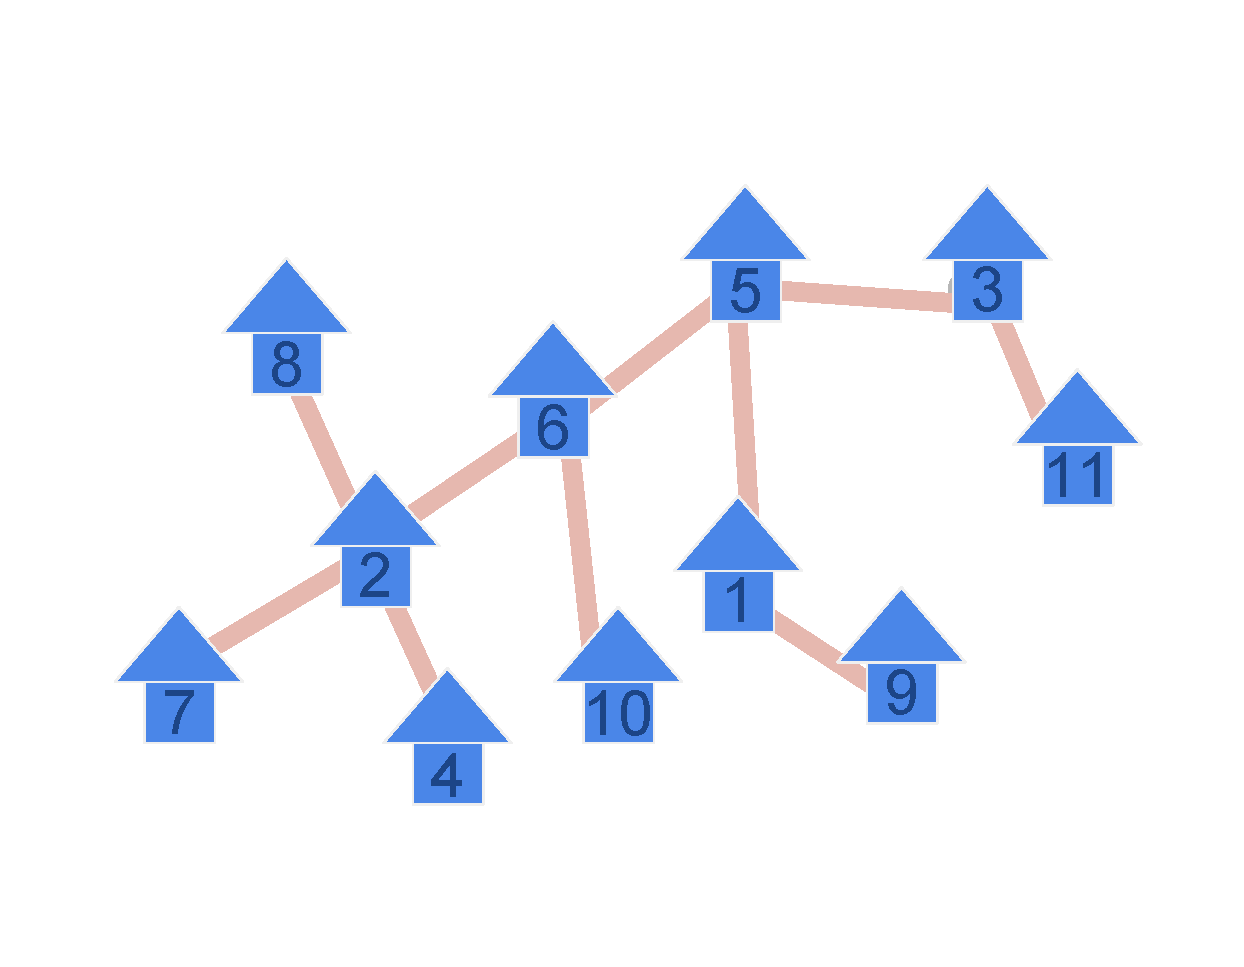
\includegraphics[scale=\termimgscale]{../img/1_infinite_loop.pdf} %\tnote{../img/1_infinite_loop.png} 
    \begin{block}{}
      {\residenceblock} residential block $\rightarrow$ \alert{\sc
        Target tree}
    \end{block}
  }

  \only<4>{
    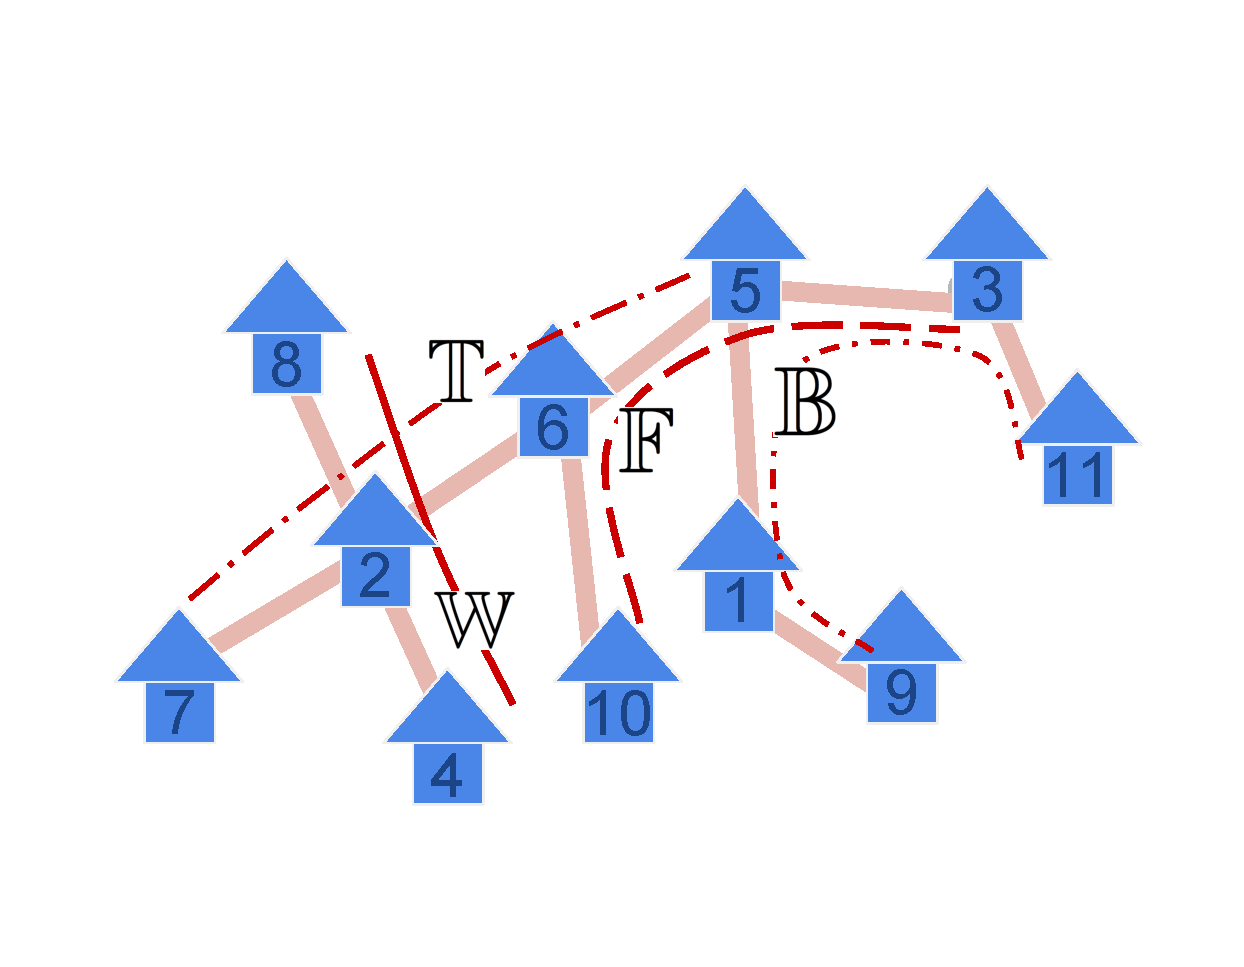
\includegraphics[scale=\termimgscale]{../img/2_infinite_loop_BTWF.pdf} %\tnote{../img/2_infinite_loop_BTWF.png} 
    \begin{block}{}
    Study group path allocation $\rightarrow$
      \alert{\sc Tree Path Labeling}

    \end{block}
  }

  \only<5,6>{
    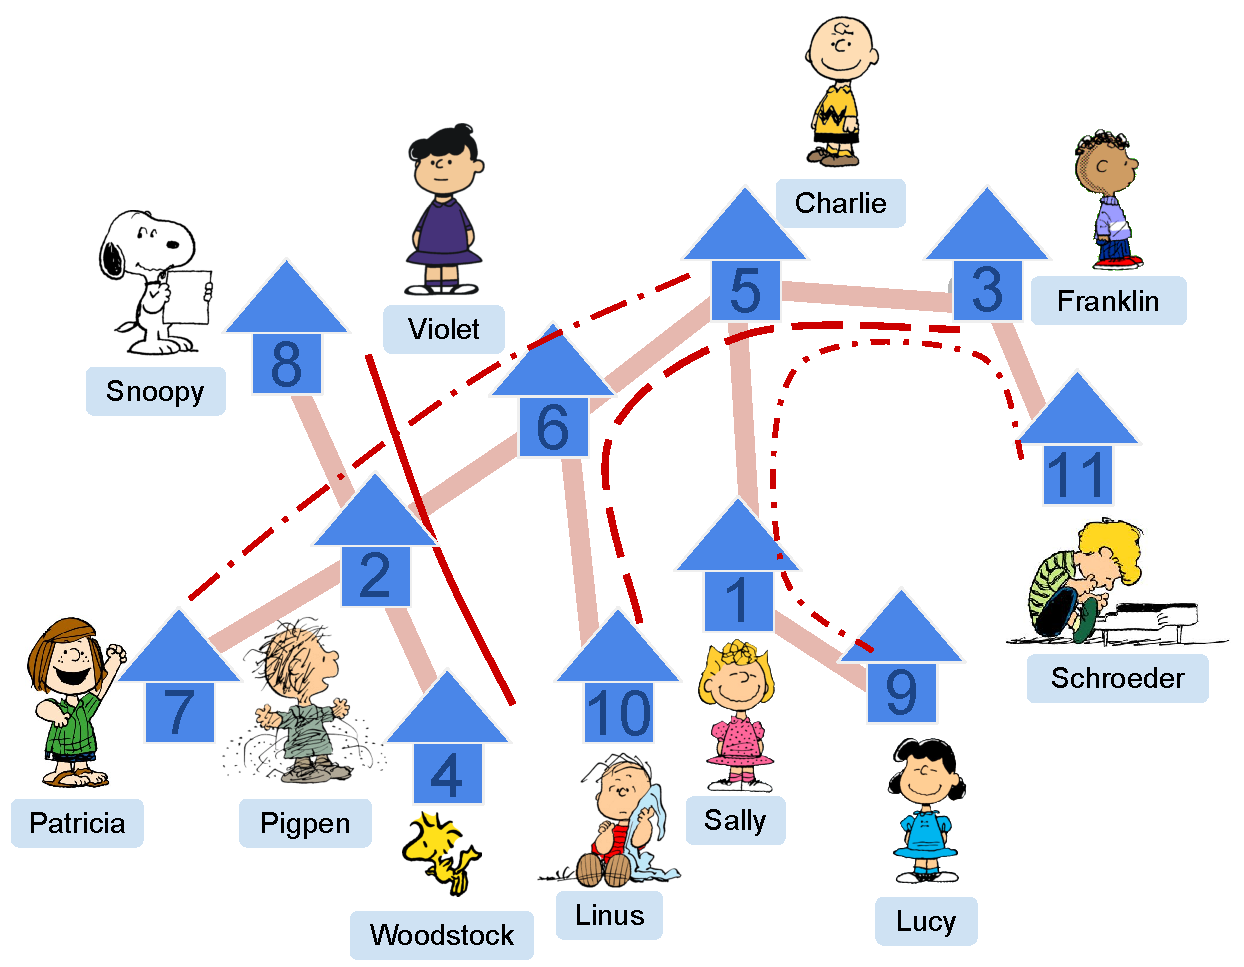
\includegraphics[scale=0.2]{../img/3_infinite_loop.pdf} %\tnote{../img/3_infinite_loop.png} 
    \begin{block}{}
      The apartment allocation $\rightarrow$ \alert{\sc Path
        Hypergraph Isomorphism} 
      
%       \only<6>{If exists, then TPL is a
%         \alert{\sc Feasible Tree Path Labeling}}
    \end{block}
  }
}


% \def\overlayht{4cm}

% \frame<1-6>{
%   \frametitle{Tree Path Labeling of Set Systems}
%   \framesubtitle{The combinatorial problem} 

%   \tnote{DELETE.}
%   \begin{block}{Terminology [contd.]}
%     \begin{overlayarea}{\textwidth}{\overlayht} 
%       \only<1>{There {\em exists} an apartment allocation that
%           ``fits'' the route mapping }
%       \only<2->{There {\em exists} a
%           \alert<2->{hypergraph isomorphism} that ``fits'' the
%           \alert<2->{TPL}\\}
%       \only<3->{$\rightarrow$ the TPL is \alert<3->{\sc feasible}\\}

%       \only<4->{There {\em exists} \only<4>{an apartment
%           allocation}\only<5->{\alert<5-> {a hypergraph isomorphism}} that
%           gives \only<4>{the optimal route mapping}
%       \only<5->{\alert<5->{paths/adjacent vertices in tree}\\}} 
% %       \only<4>{There {\em exists} an apartment allocation that
% %       gives the optimal route mapping}
% %       \only<5-> {There {\em exists} a
% %       \alert<5->{hypergraph isomorphism} that gives 
% %       \alert<5->{paths/adjacent vertices in tree}\\}
%       \only<6->{$\rightarrow$ the hypergraph is a \alert<6->{\sc
%        path hypergraph}}
%       \end{overlayarea}
%   \end{block}
% }

\def \kstar {$k$-subdivided star}
\def \FTPL {{\sc Feasible Tree Path Labeling}}
\def \CFTPLKSTAR {\sc Compute $k$-subdivided Star Path Labeling}
\def \CFTPL {\sc Compute Feasible Path Labeling} 

\frame[label=FR_PROBLEMS]{
  \frametitle{The problems studied}
%  \framesubtitle{Tree path labeling of path hypergraphs}

  \begin{block}<1,2>{1. \CFTPL} %<1->
    {\alert{Computation} of a feasible tree path labeling (FTPL) if
      any.}

    \only<2>{}

  \end{block}

  \begin{block}<1,3>{2. \CFTPLKSTAR} %<2->
    {\alert{Computation} of an FTPL if any, if target tree is a
      \alert{$k$-subdivided star}.}
  \end{block}

  \begin{block}<1,4>{3. \FTPL} %<3>
    {\alert{Characterization} of an FTPL and finding
      the feasibility bijection/hypergraph isomorphism} 
  \end{block}

}

%\subsection{Definitions}

% \frame<1>[label=intro:q1]{
% \tnote{DELETE}
% %\frame<1,9>[label=intro:q1]{
% % 1   : display normal
% % 9   : TBD defined prelim
% % 2-7 : each TBD definition highlight
% % 8   : misc definition highlight
%   \begin{center}
%     {\Huge 1}
%   \end{center}
%     \begin{block}{Characterization of feasible TPL}
%     Given
%     \begin{enumerate}[i. ]
%     \item a \textcolor<9>{\alertseccolor}
%            {\alert<2>{set system or hypergraph}} $\cF$,
%     \item a \textcolor<9>{\alertseccolor}
%            {\alert<3>{feasible} \alert<4>{TPL}} $\cl:\cF \rightarrow
%       \cP$ where $\cP$ is a path system from tree $T$ and $
%       \textcolor<9>{\alertseccolor}{\alert<5,2>{supp(} \cP \alert<5,2>{)}} = V(T)$,
%     \end{enumerate}
%     \uline{what is the \textcolor<9>{\alertseccolor}{\alert<6>{hypergraph
%         isomorphism}}} \[\underline{\phi: \supp{\cF} \rightarrow
%       \supp{\cP}}\] \uline{such that the
%       \textcolor<9>{\alertseccolor}{\alert<7,4>{induced labeling}}} 
%     $\underline{\cl_\phi = \cl}$?
%   \end{block}

%   \note[item]<9>{to understand this these will be defined in the
%     following slides}
%   \note[item]<2>{first we'll see what a set system or hypergraph is}
%   \note[item]<6>{Next is hypergraph iso}
%   \note[item]<4>{tree path labeling}
%   \note[item]<3>{feasibility of TPL}
% }

% \againframe<2>{intro:q1}

% \frame<1-3>{
%   \frametitle{}
%   \begin{definition}[Set system, Support of set system] 
%    The set $\F \subseteq (2^{U} \setminus
% \emptyset)$ is a \alert {set system} of a universe $U$ with $|U| = n$.\\

%    The \alert {support of a set system} $\F$ is
%     the union of all the sets in $\F$.\\ 
%    $ \ \ \ \ \ \ \ \ \ \ \ \ \ \ \alert{supp(\F) = \bigcup_{S \in \F}S}$
%   \end{definition}

%   \note[item]<1>{}

%   \begin{definition}<2->[Hypergraph] 
%   A \alert{hypergraph} is exactly same as a graph except that an
%   ``edge'' can have more than two
%   vertices and are called \alert{hyperedges}.
%   \end{definition}

%   \note[item]<2>{}

% %  \begin{block}<3>{} 
% %   $\cF$ can be \alert<3>{ visualized as a
% %       hypergraph} -- \alert<3>{ vertex set is $supp(\cF)$}, \alert<3>{ hyperedges are the sets
% %       in $\cF$.}
% % \end{block}

%   \only<3>{ 
%   $\cF$ can be \textbf{visualized as a
%       hypergraph} -- \textbf{vertex set is $supp(\cF)$},
%     \textbf{hyperedges are the sets 
%       in $\cF$.}
%    }

%   \note[item]<3>{}

% %   \begin{block}{Definition}
    
% %   \end{block}
% }

% \againframe<6>{intro:q1}

% \frame{
%   % \frametitle{}
%   \begin{definition}<1->[Hypergraph isomorphism \cite{kklv10}]
  
%     Two hypergraphs $\cF'$, $\cF''$ are said to be isomorphic,
%       \alert{ $\cF' \cong \cF''$}

%   $\ \ \ \ \ \ \ \ \ \ \ \ \ \ \ \ \ \ \ \ \ \ \ \ \ \ \ \ \ \ \ \ \ \
%   \Longleftrightarrow$        
 
%   there \alert{ exists a 
%     bijection $\phi: supp(\cF') \rightarrow supp(\cF'')$} s.t. \\

%     \alert{   for
%     all sets $A \subseteq supp(\cF')$
% $A \in \cF'$ $\Leftrightarrow$
%     $B \in \cF''$ where $B = \{\phi(x) \mid x \in
%     A\}$}, written as $B=\phi(A)$.
%   \end{definition}
% }

% \againframe<4>{intro:q1}

% \frame{
% %  \frametitle{Tree path labeling (TPL)}

%   \begin{overlayarea}{\textwidth}{5cm}
%   \begin{definition}<1->[Tree Path Labeling (TPL)]
%     For a set system $\cF$, \alert{$\cl: supp(\cF) \rightarrow \cP$} where
%     $\cP$ is a set of paths from $T$, is called a \alert{TPL} if their
%     intersection graphs are isomorphic \textcolor<2->{contrast}{(not
%       hypergraph isomorphism)} \alert{$\bI(\cF) \cong \bI(\cP)$},
%     $\cl$ is the isomorphism.\\
 
%    Alternate notation for the \alert{path representation} $\cP$ is \alert{$\cF^\cl$}.
%   \end{definition}
%   \only<2>{i.e. intersection properties are preserved. but {\bf not}
%     necessarily intersection cardinality properties.}
%   \end{overlayarea}
%   \begin{definition}<3->[Induced TPL]
%    If $\cF \cong \cP$ \textcolor<4>{contrast}{(hypergraph
%      isomorphism)} and $\phi$ is the isomorphism $\Longrightarrow$
%    this induces a path labeling. This is called \alert{induced path
%      labeling, $\cl_\phi$}
    
%   \end{definition}

% }

% \againframe<3>{intro:q1}

% \frame{
% %  \frametitle{Feasible labeling}

%   \begin{definition} [Feasible TPL]
%     A TPL $(\cF, \cl)$ is defined to be \alert{feasible} if
% % $\cF \cong \cF^\cl$ and this
% there is \alert{a hypergraph isomorphism $\phi: supp(\cF) \rightarrow
% supp(\cF^\cl)$} $=V(T)$ which induces path labeling $\cl_\phi: \cF \rightarrow
% \cF^\cl$ such that \alert{$\cl_\phi = \cl$}.
%   \end{definition}

%   \only<2->{ Recall:
%     \begin{itemize}
%     \item<2-> $\cF \cong \cF^\cl$ and $\phi$ is the \textbf{hypergraph
%         isomorphism}
%     \item<3-> $\bI(\cF) \cong \bI(\cF^\cl)$ and $\cl$ is the \textbf
%       {graph isomorphism}
%     \item<4-> \textbf{and} the induced TPL $\cl_\phi$ must be same as $\cl$.
%     \item<5-> If there is such a $\phi$ then $\cl$ is feasible.
%     \end{itemize}
%   }

% }

% \frame<1>[label=intro:q2]{
% %\frame<1-2>[label=intro:q2]{
%   \tnote{DELETE}
%   \begin{center}
%     {\Huge {\tt 2}}
%   \end{center}
%   \begin{block}{Computing a feasible TPL}
%     Given hypergraph $\cF$ with certain properties and a
%     \alert<2>{$k$-subdivided star} $T$, \uline{can we find a feasible TPL 
%       $\cl$ to $T$?}
%   \end{block}
% %  \note{}
% }

% \frame {
% %  \frametitle{$k$-subdivided star}

%   \begin{definition}[$k$-subdivided star]
%     A \alert{$k$-subdivided star} is a star with all its edges
%     subdivided exactly $k$ times.
%   \end{definition}

%   \only<2>{ \includegraphics[scale=0.5]{star.pdf} $k = 0$ }
%   \only<3>{ \includegraphics[scale=0.5]{kstar.pdf}  $k = 2$}

%   \note{we'll see details later.}
% }

% %\againframe<1>{intro:q2}

% \frame{
%   {\center We will see the problems in LIFO order - more specific to general.}
% }

\section{Results}

 \frame {
  
    {\Huge 3.}
   \begin{block}<2>{Characterization}
     \begin{itemize}
     \item Three way intersection cardinality preservation
     \item Filtering and pruning algorithm
     \end{itemize}
    \end{block}
 }



% \subsection{ICPPL}
% \frame [label=icppl:pr]{ %[label=SLIDENOW]{ % 
%   \frametitle{ICPPL - a TPL with special properties}
%   \framesubtitle{Intersection Cardinality Preserving Path Labeling}

% %  \tnote[a]{TBD list ICPPL properties}
% %  \note{}
% }

% \frame<1> [label=th:icpplth]{ % [label=SLIDENOW]{ % 
%   \frametitle{The characterization}
%   \framesubtitle{ICPPL + a filtering algorithm}

%   \tnote[a]{TBD Write the theorem}
% %  \note{}
% }

% \subsection{Filtering algorithm}
% \frame [label=flow:filtering]{ %[label=SLIDENOW]{ %
%   \frametitle{The filtering algorithm}
%   \framesubtitle{{\tt filter\_1}\\ 
%                  {\tt filter\_2}\\ 
%                  Algorithm {\tt get-hypergraph-isomorphism}}

%   \tnote[a]{TBD flow chart of the filtering algorithm. see notes.}
% %  \note{}
% }

% \frame [label=al:filter1]{ %[label=SLIDENOW]{ %
%   \frametitle{\tt filter\_1}
%   \framesubtitle{Make leaves unique to paths} 

%   \tnote[a]{TBD present the algorithm with images? with psuedocode on
%     the side? f yeah. like dessert. apple pie with cream on the side please.}
% %  \note{}
% }

% \frame [label=al:filter2]{ %[label=SLIDENOW]{ %
%   \frametitle{\tt filter\_2}
%   \framesubtitle{Find elements that map to leaves}

%   \tnote[a]{TBD present the algorithm with images? with psuedocode on
%     the side? f yeah. like dessert. apple pie with cream on the side
%     please.} 
% %  \note{}
% }

% \frame [label=al:treeprune]{ %[label=SLIDENOW]{ %
%   \frametitle{Algorithm {\tt get-hypergraph-isomorphism}}
%   \framesubtitle{Find hypergraph isomorphism $\phi$ - recursively use
%     {\tt filter\_1} {\tt filter\_2}}

%   \tnote[a]{TBD present the algorithm with images? with psuedocode on
%     the side? f yeah. like dessert. apple pie with cream on the side
%     please.} 
% %  \note{}
% }

%\againframe<1>{th:icpplth}     % Show theorem again before proof.
%  \note{}

% \subsection{Proof and analysis}

% %\frame [label=SLIDENOW]{
% \frame [label=char:proof]{ 
%   \frametitle{Proof}
%  \framesubtitle{Outline}

%   \tnote[a]{Give outline of the proof.}
%   \note{}
% }

% %\frame [label=SLIDENOW]{
% \frame [label=char:proof]{ 
%   \frametitle{Brief analysis}
% %  \framesubtitle{Outline}

%   \tnote[a]{Give brief analysis.}
%   \note{}
% }


% \section[Computation of TPL]{Computing a feasible TPL on
%   $k$-subdivided trees} 

% \againframe<1>{intro:q2}       % Show q2 again - refresher.
% %  \note{}

%\subsection{Algorithm}

% \frame [label=SLIDENOW]{
\frame{ \frametitle{Special case} \framesubtitle{Interval assignment
    problem / COP}

  \begin{enumerate}
  \item<1-> $T$ is a path $\Longrightarrow$ paths in $T$ are intervals
    %\tnote[a]{quick illustration}
  \item<1-> Only pairwise intersection cardinality needs to be
    preserved $\Longrightarrow$ ICPIA \cite{nsnrs09}
  \item<1-> Higher level intersection cardinalities preserved by {\bf
      Helly Property} -- \cite{mcg04}
  \item<1-> {\em filter\_1},{\em filter\_2} do not need the the {\bf
      exit} conditions. 
  \end{enumerate}
  
  \begin{block}{}
    This problem is equivalent to Consecutive Ones Property of binary
    matrices \cite{nsnrs09}
  \end{block}

}

 \frame {
  
    {\Huge 2.}
  
    \begin{tabular}[h]{ccccc}
  \includegraphics[scale=0.3]{../img/star.pdf} &&&&
  \includegraphics[scale=0.3]{../img/kstar.pdf}\\
  (a) &&&& (b)
  \end{tabular}

   \begin{block}<2>{Compute TPL on $k$ subdivided stars}
     \begin{itemize}
     \item each rays of the k sub star are independent intervals when
       root is excluded.
     \item each ray is considered independently as interval
       assignment problem
     \end{itemize}
    \end{block}
 }



% %\frame [label=TEST BIBTEX]{
% \frame {
%   \frametitle{???}
%   \cite{d08phd}\\
%   \cite{bl76}\\
%   \cite{fg65}
% }


% \subsection{Proof and analysis}

% \frame [label=SLIDENOW]{ 
%   \frametitle{Proof}
%   \framesubtitle{Outline}

%   \tnote[a]{Give outline of the proof.}
%   \note{}
% }

% \frame [label=SLIDENOW]{ 
%   \frametitle{Brief analysis}
% %  \framesubtitle{Outline}

%   \tnote[a]{Give brief analysis.}
%   \note{}
% }



\section{Conclusion}
\subsection{Application}
% \frame[label=FR_APP]
% {
%     \frametitle{Path Labeling $\rightarrow$  Graph Isomorphism}
%     \framesubtitle{Application} 

%     \tnote{get a better image!}
%     \only<1>{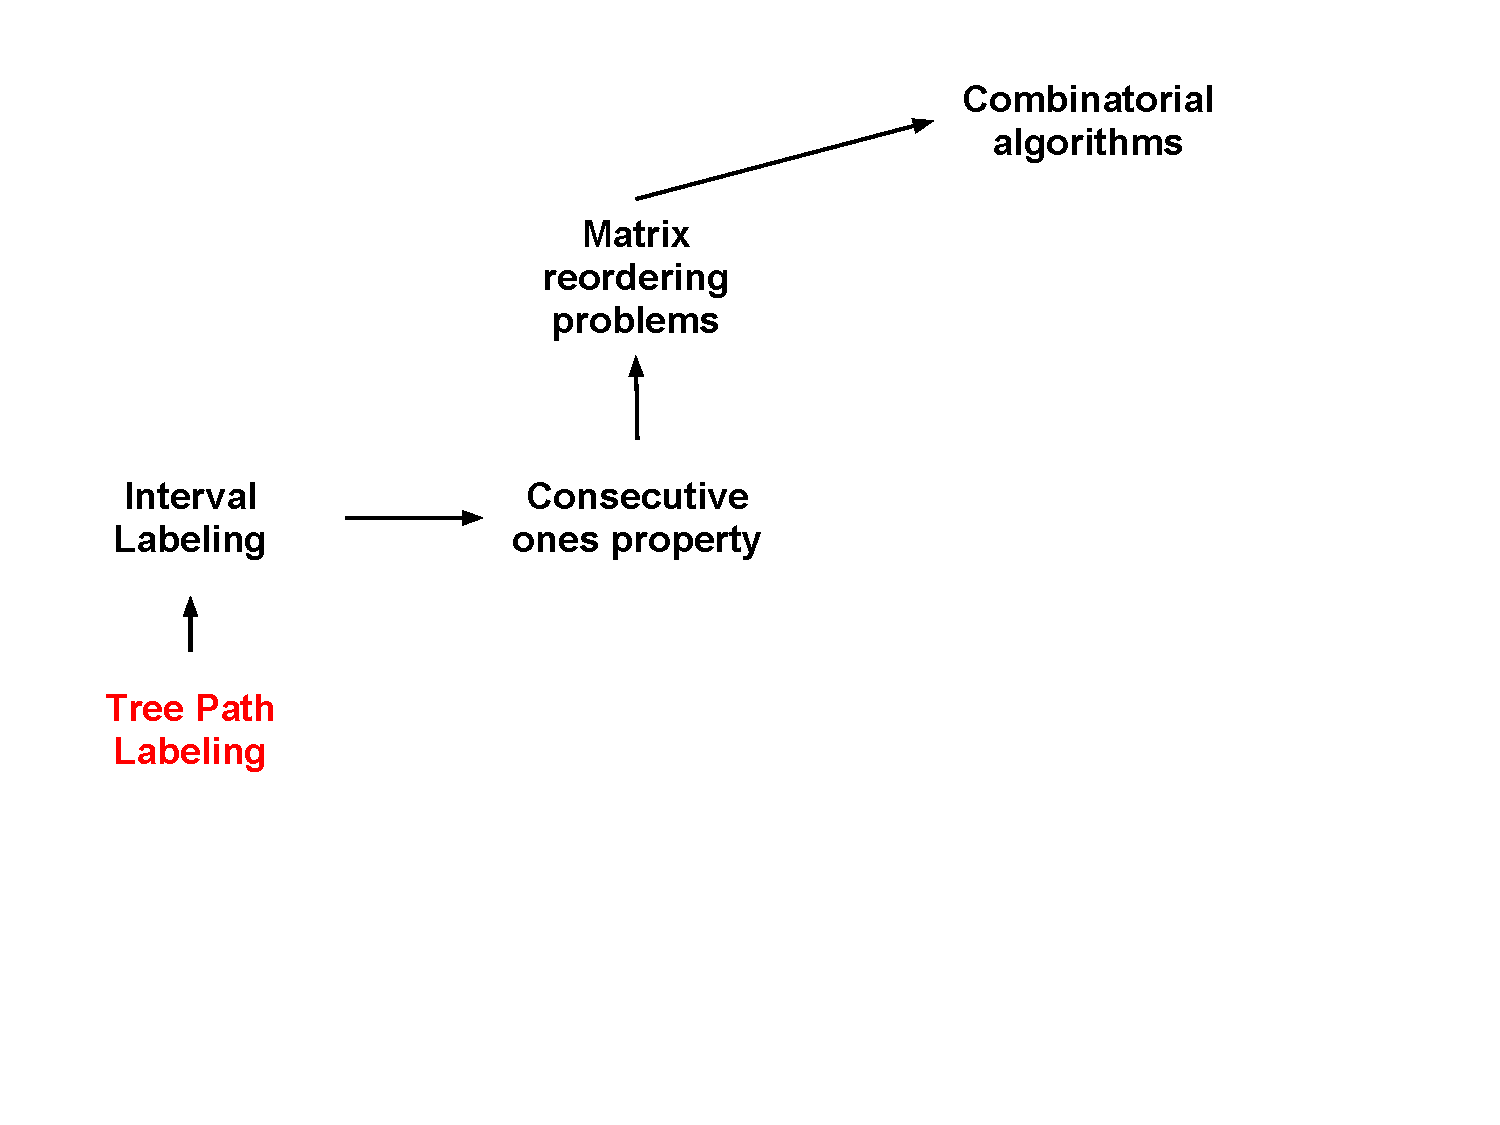
\includegraphics[scale=0.3]{m1.pdf}} 
%     \only<2>{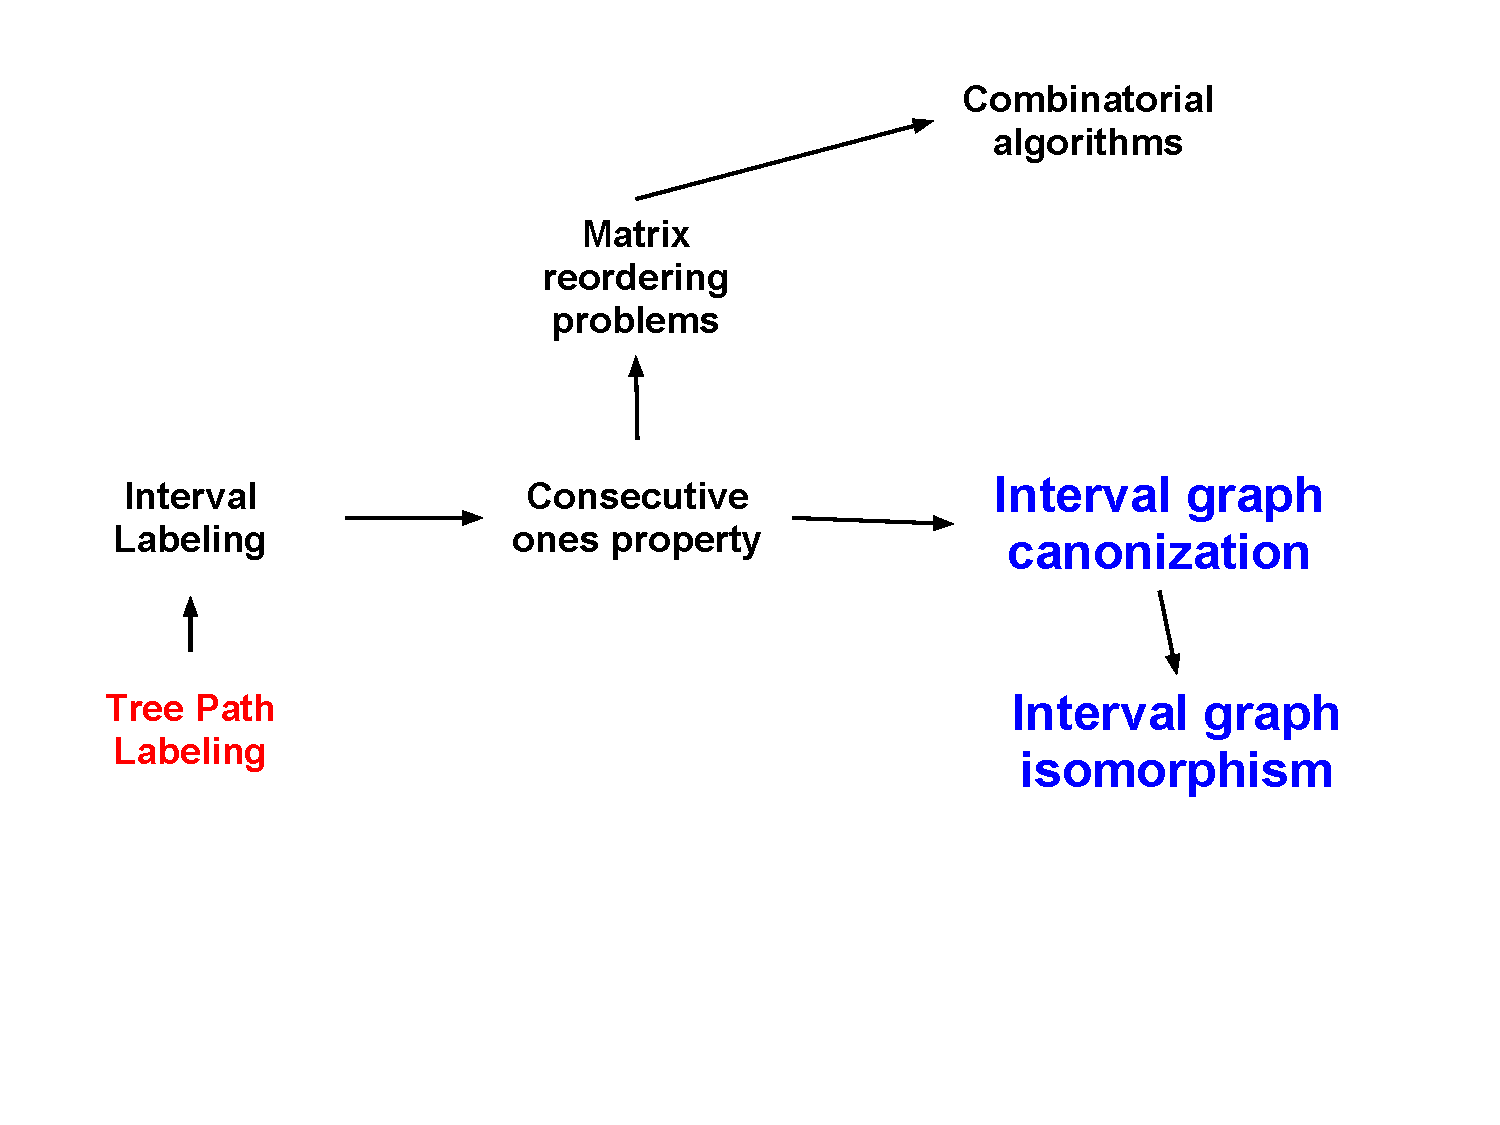
\includegraphics[scale=0.3]{m2.pdf}} 
%     \only<3>{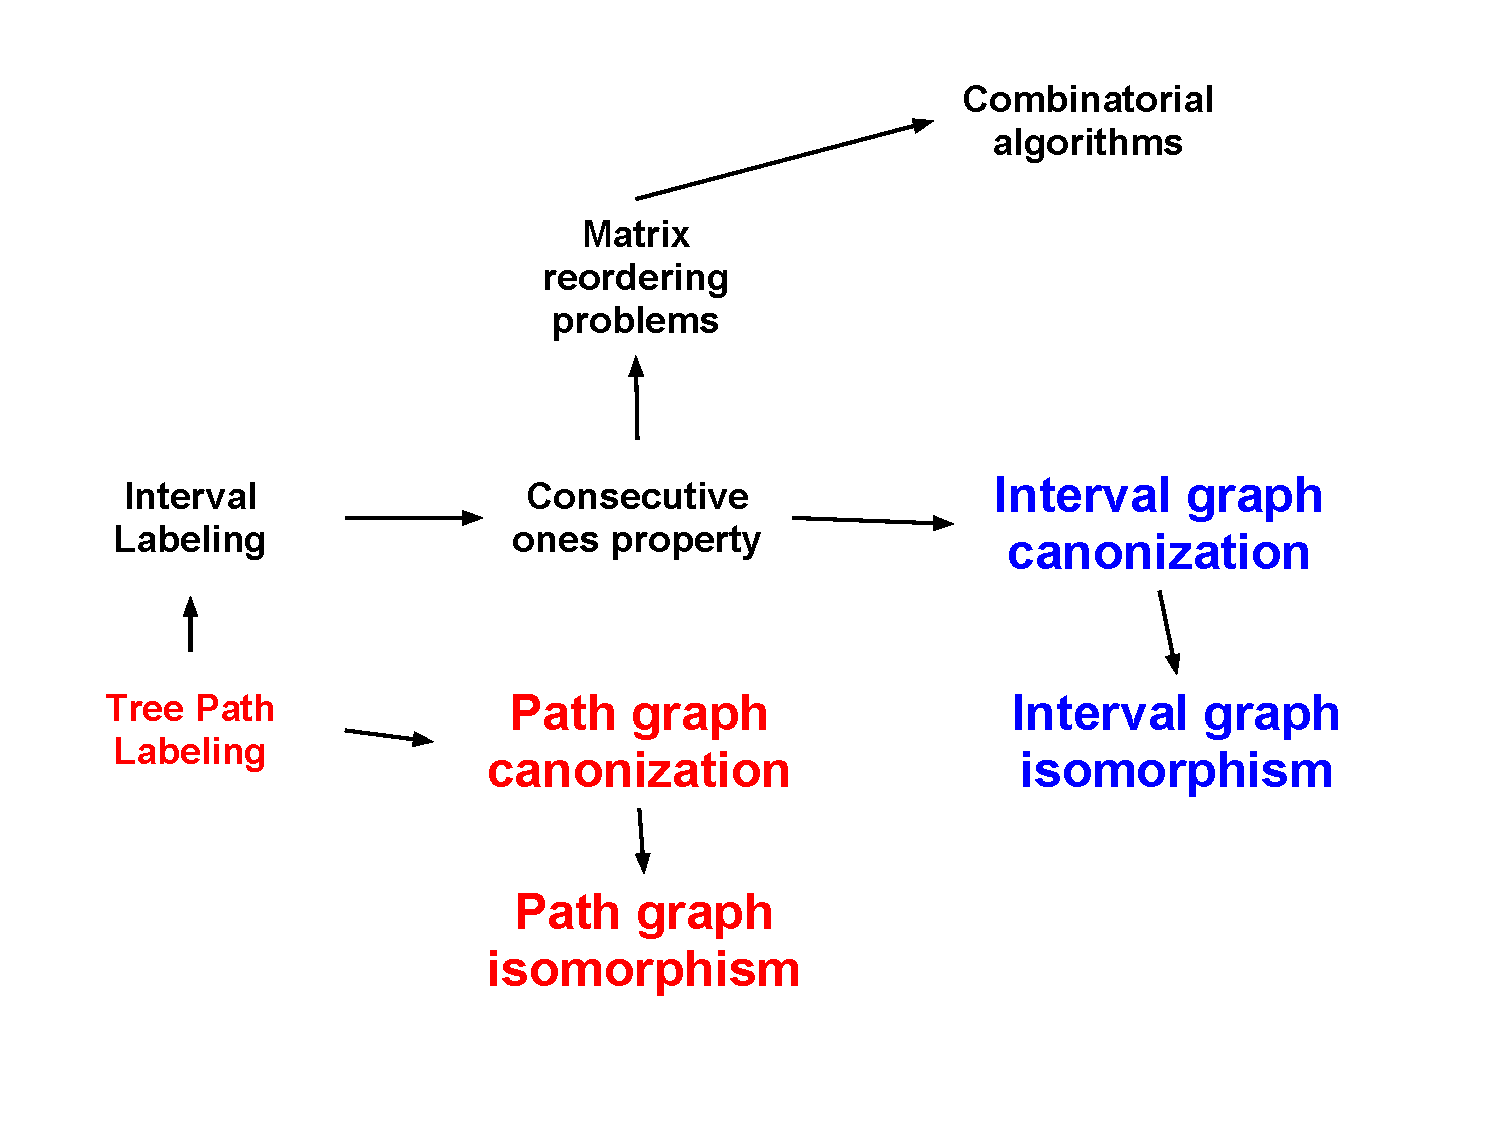
\includegraphics[scale=0.3]{m3.pdf}} 

% %    \note{}
% }

\againframe<1,2,3>{FR_MOTIVE}

\frame{
  \frametitle{Thank You}

  \begin{centering}
   Q \& A
  \end{centering}
}

\section*{References}
\frame%[allowframebreaks]{References} 
{
% \tnote{improve - add some jazz. this is a notional slide only for
%   offline reference.}
\tiny  %\footnotesize
\bibliographystyle{alpha}
\bibliography{../lib/cop-variants__thesis}
}

% \frame{
%   % TEMP: to enforce toc entries when frames haven't been decided
%   % yet. 
% } 

\end{document}
